\documentclass{pdfmx4020}
%\documentclass{mx4020}
\usepackage{hyperref}
\usepackage{amsmath,amsthm}
% Erin's additions
\usepackage{color} 
\usepackage{graphicx}
\usepackage{float}
\usepackage{algorithm2e}
\usepackage{tikz}
\usepackage{array}
\usetikzlibrary{decorations.pathmorphing}
\usetikzlibrary{decorations.fractals}

\newtheorem*{defn}{Definition}
\newtheorem*{thm}{Theorem}
\newtheorem*{exa}{Example}
\newtheorem*{no}{Note}

\Title{Particle Swarm Optimisation for the Portfolio Selection Problem in a Function Based Environment}
% \Title{Functional Approach }
\Author{Anthony S. Chapman}
\Year{2013--2014}
\Supervisor{Dr. Wei Pang}

\graphicspath{ {./Figures/} }

\begin{document}

% \mxfrontpage
\newfrontpage

% \begin{Summary}
% Summary....
% \end{Summary}

\begin{Abstract}
Abstract....
\end{Abstract}

\begin{Acknowledgments}
Acknowledgments....
\end{Acknowledgments}

\StartThesis

\chapter{Introduction}
  \section{Overview} % (fold)
  \label{sec:overview}
  
  % section overview (end)

  \section{Motivation} % (fold)
  \label{sec:motivation}
  % section motivation (end)

  \section{Primary Goals} % (fold)
  \label{sec:primary_goals}
  
  % section primary_goals (end)

  \section{Secondary Goals} % (fold)
  \label{sec:secondary_goals}
  
  % section secondary_goals (end)

\chapter{Background}\label{chap:background}
  In order to expand and adapt existing Particles Swarm Optimisation methods an initial background research has to be done to fully understand the concepts involved. Similarly to fully 

  \section{Particle Swarm Optimisation} % (fold)
  \label{sec:particle_swarm_optimisation}
    % Particle Swarm Optimisation (PSO) \cite{pso,pso2,pso3,pso4} is a metaheuristic inspired on the social behavior of flocks of birds when flying and on the movement of shoals of fish. A population of entities moves in the search space during the execution on the algorithm. These entities perform local interactions (with other particles as well as the environment).

    % Assuming worker bees are searching for a patch of flowers with the most pollen, also assume that the bees

  Particle swarm optimization (PSO) is a population based  stochastic optimization technique developed by Kennedy and  Eberhart in 1995, discovered through simplified social model simulation \cite{pso,pso2,pso3,pso4}. It simulates the behavior of bird flocking involving the scenario of a collection of birds randomly looking for food in a search space. None of the birds know where the food is located, but they do know how far the food location is from their current positions. An effective technique for the bird to find food is to adjust their velocity according to the bird which is nearest to the food. PSO was motivated from this scenario and was developed to solve complex optimization problems, where the optimum position of the fitness function is where the food is located and all the birds are the particles searching for this optimum position. 

  In the conventional PSO, the behaviour displays particles in a multidimensional space where each particles has two properties: a position vector and a velocity vector. Each particle $i$ in the swarm has the properties shown in (\ref{eq:PSO_stuff}):
    % \begin{itemize}
    %   \item $X_i^k$ : The current position of particle i at time k.
    %   \item $V_i^k$ : The current velocity of particle i at time k. 
    %   \item $Pbest_i^k$ : The personal best position of particle i at time k. 
    %   \item $Gbest^k$ : The global best position of particle i at time k. 
    % \end{itemize}
    \begin{equation} \label{eq:PSO_stuff}
      \begin{split}
        & V_i^t \text{ : The velocity of particle i at time t.} \\
        & X_i^t \text{ : The current position of particle i at time t.} \\
        & Pbest_i^t \text{ : The personal best position of particle i at time t.} \\
        & Gbest^t \text{ : The global best position of particle i at time t.} \\
      \end{split}
    \end{equation}

    At each step, the velocity of the $ith$ particle will be updated according to the following equation:

    \begin{equation} \label{eq:vel}
      \begin{split}
        V_{i}^{t+1} & = \omega V_{i}^{t} + c_1 r_1 \times \Big( Pbest_{i}^{t} - X_{i}^{t} \Big) + c_2 r_2 \times \Big( Gbest^{t} - X_{i}^{t} \Big) \\
        \text{where} & \\
        & V_i^{t+1} \text{ : The velocity of particle i at time t + 1.} \\
        & V_i^t \text{ : The velocity of particle i at time t.} \\
        & X_i^t \text{ : The current position of particle i at time t.} \\
        & \omega \text{ : Inertia weight parameter.} \\
        & c_1, c_2 \text{ : Acceleration coefficients.} \\
        & r_1, r_2 \text{ : Random numbers between 0 and 1.} \\
        & Pbest_i^t \text{ : The personal best position of particle i at time t.} \\
        & Gbest^t \text{ : The global best position of particle i at time t.} \\
      \end{split}
    \end{equation}

  In the updating process shown in Equation (\ref{eq:vel}) the acceleration coefficients $c_1, c_2$ ($c_1$ determines the importance one following the individual personal best whereas $c_2$ determines the importance of following the particles with the global best position)and the inertia weight $\omega$ (which states how stubborn a particle is at not deviating from their path, regardless of previous results) are predefined, and $r_1, r_2$ (these introduce the concept of randomness so that a particles is able to switch between following their personal best and that of the whole swarm) are uniformly generated random numbers in the range [0,1].

    \begin{algorithm}[H] \label{eq:pso}
      \mbox{\textbf{Initialisation}} \\
      \For{i = 1,\dots,S}{
        initPosition(i) \\
        initBestLocal(i) \\
        \If{i = 1}{initBestGlobal()} 
        \If{improvedGlobal(i)}{updateGlobalBest(i)} 
        initVelocity(i)
      }
      \mbox{\textbf{Main program}} \\      
      \While{not endingCondition()}{
        \For{i - 1,\dots, S}{
          createRnd($r_1,r_2$) \\
          updateVelocity(i$,r_1,r_2$) \\
          updatePosition(i) \\
          \If{improvedLocal(i)}{updateBestLocal(i)}
          \If{improvedGlobal(i)}{updateGlobalBest(i)}
        }
      }
      \caption{PSO pseudo-code.}
    \end{algorithm}
  
  In Algorithm~\ref{eq:pso} $S$ is the number of particles in a swarm, one can see the pseudo-code for a standard PSO. A step by step explanation of Algorithm~\ref{eq:pso} is as follows: First, there is an initialisation for all the particles in the PSO, for every particle $i$, \textit{initPosition(i)} randomly created a particle with a designated position in the search space. For the first step, \textit{initBestLocal(i) = initPosition(i)}, but it will be updated afterwards. Then the $if$ function makes a first global best and if any other particles has a better global best position it will be set as the new global best. \textit{initVelocity(i)} gives particle $i$ an initial velocity which is randomly generated. 

  After the initialisation, the core of the PSO method is executed until the \textit{endingCondition()} is satisfied, which can be the number of iterations or an improvement threshold. In the body of the \textit{While} loop all particles are updated. The first step is to generate random numbers used in the velocity Equation~(\ref{eq:vel}). Then the actual velocity is updated. In the next step,\textit{updatePosition(i)} updates the position of a particles in the search space and checks the fitness function value for improvement or not. At the end of the \textit{for} loop, if \textit{improvedLocal(i) = True} then updates the local best position and finally it is similar for updating the global best position. 
  % section particle_swarm_optimisation (end)

  \section{Portfolio Optimisation} % (fold)
  \label{sec:portfolio_management}
  The term portfolio refers to a collection of investments such as stocks, bonds or other securities \cite{portfolio}. For this project we will focus on stocks but it would be trivial to include other such securities into the application as they behave in a similar manner to stocks. Portfolio Optimisation is the process of choosing the proportion of various assets to be held in a portfolio in such a way that any other choice would result in an equal or worst portfolio, here we have referred to the comparison of portfolio from the rate of return or the level of risk, ie one portfolio is better than another if it has a lower level of risk or higher rate of return. 

  This paper will focus on the two-sided coherent risk measure introduced in \cite{two_sided_risk}. This revolutionises how to calculate risk as it takes into account both downside as well as upside risk in unison. Compared to previous risk measures this new measure has the following advantages:
  \begin{itemize}
    \item The whole domain loss distribution information is utilised, making it superior for finding robust and stable investment decisions.
    \item Suitably selecting the combination coefficient and the order of the norm of the downside random loss, it is easy reflect the investor's risk attitude and to control the asymmetry and fat tails of the loss distribution.
    \item It is easy to compute and therefore easier to apply to optimisation models.
  \end{itemize}

  Now this is where some mathematical background is needed, let $\| X \|_p = (E_Q |X|^p)^{\frac{1}{p}}$, $\|X\|_\infty = ess.sup \{ |X|\}$, $\sigma_p^{\pm} (X) = \|(X-E_Q[X])^{\pm}\|_p$. As already mentioned, this two-sided risk measure takes into account both sides of the loss distribution, so relative to the expected return value $E_Q[X]$, the random variable $(X-E_Q[X])^-$ is the ``downside risk'' of $X$, which according to \cite{two_sided_risk} might be more crucial to an application than the analogues ``upside risk'' variable $(X-E_Q[X])^+$.

  Due to the way downside and upside risk can be represented and the monotonically increasing property of $\| \cdot \|_p$ with respect to p, two-sided risk measure can be determined by the following equation:
  \begin{equation} \label{eq:two-sided}
    \begin{split}
      & \text{For } 1 \leq p \leq \infty \text{ and } a \in [0,1] \\
      \rho_{a,p}(X) & = a \sigma_1^+(X) + (1-a)\sigma_p^-(X) - E_Q[X ]\\
      & = a \|(X-E_Q[X])^+\|_1 + (1-a) \|(X-E_Q[X])^-\|_p - E_Q[X] \\
    \end{split}
  \end{equation}


  $\rho_{a,p}(X)$ in Equation~\ref{eq:two-sided} is generated by first taking the 1-norm of the positive deviation and the $p$-norm of the negative deviation and then taking the combination of these two norms. The inclusion of $- E_Q[X]$ in Equation~\ref{eq:two-sided} ensures that $\rho_{a,p}(X)$ is coherent \cite{two_sided_risk}. 

  One of the advantages proposed for two-sided coherent risk measure was that it would be easy to reflect an investor's attitude towards risk, this is achieve by the variables $p,a$ in $\rho_{a,p}(X)$ in Equation~\ref{eq:two-sided}. An investor's risk adverse attitude is represented by $p$, where the larger $p$ is, the more risk the investor is willing to take, so small $p$ low risk, large $p$ high risk. In Equation~\ref{eq:two-sided} $a$ is the factor controlling the balance between good and bad volatility \cite{two_sided_risk} where $a \to 0$ represents an investors attitude towards good volatility where $a \to 1$ does the converse. Thus different inverstors might choose different values for $p$ and $a$.

  A reader might not see how Equation~\ref{eq:two-sided} has much to do with calculating risk from a first glance, a quick example will be shown to illustrate it's use. Suppose we have $N$ assets to choose from and for $i \in [1,N]$ let $x_i \in [0,1]$ be the proportional weight of asset $i$ in the portfolio, let $r_i \in \R$ be a variable which represents the rate of return of asset $i$ and $\widehat{r}_i$ be the expected return of asset $i$. Then the rate of return of a portfolio can be expressed as $R = \sum_{i=1}^N x_i r_i$ and the expected return $\widehat{R} = \sum_{i=1}^N  x_i \widehat{r}_i$

  From Equation~\ref{eq:two-sided} we can measure the risk of a portfolio as follows:
  \begin{equation} \label{eq:portfolio-risk}
    \begin{split}
      \rho_{a,p}(R) & = a \|(R-\widehat{R})^+\|_1 + (1-a)\|(R-\widehat{R})^-\|_p - \widehat{R} \\
    \end{split}
  \end{equation} 
  Now that there is a way to measure risk, the portfolio optimisation problem can be formulated as follows:
  \begin{equation} \label{eq:portfolio-risk-min}
    \begin{split}
      \text{min } \rho_{a,p}(R) \\
    \end{split}
  \end{equation} 
  Subject to constraints:
  \begin{equation} \label{eq:portfolio-risk-constraints}
    \begin{split}
      \widehat{R} = \eta \\
      \sum\limits_{i=1}^N x_i = 1 \\
      l_i \leq x_i \leq u_i
    \end{split}
  \end{equation} 

  Equation~\ref{eq:portfolio-risk-min} refers to the minimisation of a portfolio's risk. Now an explanation for the constraints in Equation~\ref{eq:portfolio-risk-constraints}, $\eta$ is the required rate of return of a portfolio, that is what the investor has to gain, this constraint ensures that the portfolio reaches this return. The sum of $x_i$ ensures the investors do not buy more than what they can afford and also that the investor invests all the capital it can. Finally, $l_i$ and $u_i$ are lower and upper limits for how much proportion of each asset an investor is allowed to invest in, this is useful for diversification. 

  % section portfolio_management (end)
  

  \section{Haskell} % (fold)
  \label{sec:haskell}
  This section briefly introduces the main attractions of the functional language Haskell. One big advantage of pure functional programming languages is that the absence of side-effects provides a clear semantic framework to analyse the correctness of programs and algorithms. The core notion of functional programming is that everything is a mathematical function, so everything has an input and an output, similarly to object orientated languages, where everything is an object. This is not exactly clear, to make it simpler, in Haskell, everything is a function or a variable, but something it can be both! By this I mean we can apply function composition. One can think of this by having a function and to that function you can input another function and the output could either be yet another function or a value. 

  ``Real World Haskell'' by Don Stewart, Bryan O'Sullivan, and John Goerzen is a brilliant book to quickly get your head around Haskell. Having a very strong mathematical background I often struggled to understand or accept very simple concepts in object-orientated languages such as Java or Ruby. Once Haskell was introduced to me, there was no going back.

  Back to our project, Haskell is one of the leading lazy evaluation languages in the functional programming community \cite{lazy}. Lazy evaluation, if you did not know, is an evaluation strategy which delays the evaluation of each expression until the exact moment when it is actually required, this is indeed a powerful tool. Haskell is also a strongly typed language which includes polymorphism and high-order programming facilities. 

  ---------------More why it's good for this specific project --------------

  % section haskell (end)

  % \section{Multi-objective Optimisation} % (fold)
  % \label{sec:multi_objective_optimisation}
    
  % % section multi_objective_optimisation (end)


\chapter{Related Work}
  \section{Markowitz Model} % (fold)
  \label{sec:markowitz_model}
    One of the first contributions to the portfolio problem was made by Markowitz \cite{marko1} which was later described in more detail in his book \cite{marko2}. Markowitz introduced the mean-variance model which considers the variance of the portfolio as the measure of the investor's risk under a set of assumptions. According to Markowitz, the portfolio selection problem can be expressed as an objective function subject to linear constraints. 

    Following Markowitz, the investment horizon includes a single period whereas the investment strategy is to select an optimal portfolio at the beginning of the period which will be held unchanged until the date of termination. The joint distribution of one-period security returns is assumed to be a multivariate normal distribution, which in turn follows that the distribution of the portfolio return is also normal. 

    Let $S = (S_1,S_2,S_3, \dots , S_N)$ be the set of $N$ assets where each asset $S_i$ has a rate of return represented by a variable $R_i$ with an expected return $r_i$ and each pair of assets $(S_i,S_j)$ has a covariance $\sigma_{ij}$ . The variance-covariance matrix $\sigma_{n\times n}$ contains all the covariance values, furthermore, it is a symmetric matrix and every diagonal element $\sigma_{ii}$ represents the variance of asset $S_i$. Let $\pi$ be a positive value which represents the investor's required expected return. Generally the values $r_i$ $\sigma_{ij}$ are estimated from past data and are fixed during the period of investment. 

    According to Markowitz, a portfolio is a real valued vector $X = (x_1,x_2,x_3, \dots ,x_i)$ where each variable $x_i$ represents the percentage invested in a corresponding asset $S_i$. The value $\sum\limits_{i=1}^N \sum\limits_{j=1}^N x_i x_j \sigma_{ij}$ is the variance of the portfolio and it is the measure of risk associated with the portfolio. From this, we may obtain a constrained portfolio optimisation problem: 
    \begin{equation}
      \begin{split}
        \mbox{\textit{Minimise  }} \sum\limits_{i=1}^N \sum\limits_{j=1}^N x_i x_j \sigma_{ij} \\
        \\\\
        \mbox{\textit{Constraints:} }
        \sum\limits_{i=1}^N x_i r_i = \pi \\
        \sum\limits_{i=1}^N x_i = 1 \\
        x_i \geq 1, i \in \{1,2,\dots,N\}
      \end{split}
    \end{equation}

    Here, the objective function minimises the total variance (risk) associated with a portfolio whilst the constraints ensure that the portfolio meets the expected required return of $\pi$ and the proportions of all the assets sum to 1. The non-negative constraint means that no short-selling is allowed. 

    This framework presumes that the investor uses a quadratic utility function or that asset returns follow a multivariate normal distribution. This implies that the rate of return of a portfolio of assets can be completely explained by the expected return or variance of assets. The efficient-frontier is the set of assets which provide minimum risk for a specified level of return. Solving the Markowitz portfolio optimisation problems for different specified expected portfolio returns will give us a set which represents the efficient-frontier, it is a smooth semi-increasing curve which represents the best possible trade-off between risk and expected return, also called the set of Pareto-optimal portfolios \cite{pareto}. 

    \begin{figure}[H]
      \centering
        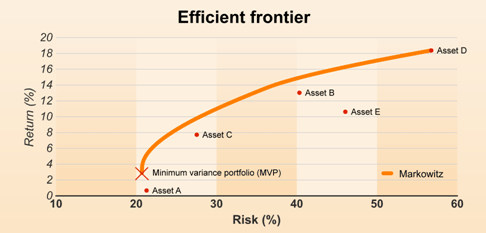
\includegraphics[width=0.9\textwidth]{efficient_frontier}
      \caption{Example of an Efficient Frontier Without a Risk-Free Asset \cite{efficient_frontier}.}
      \label{efficient_frontier}
    \end{figure}

    Each point on the line in Figure~\ref{efficient_frontier} represents a portfolio which is considered to be efficient (ie no other portfolio provides higher return without more risk and similarly for risk). In Figure~\ref{efficient_frontier} Assets A-E represent what the portfolio will be made out of. 

    Markowitz's model is subject to serous criticisms as stated in \cite{crit}, and the main ones being that a measure of dispersion can be adopted as a measure of risk only if the relevant distribution is symmetric. Another problem is that the distribution of individual asset returns has a tendency to show a higher probability of being fat-tailed. In case of non-normal, non-symmetric distributions, the utility function must be quadratic \cite{crit}. 

    This criteria should not be taken lightly since the assets' return does not follow normal distributions in real world situations \cite{non-dist}. This approach can only be used if the investor's utility function is quadratic with non-positive second derivatives or if the asset's return distribution can be fully described. Several research have indicated that that the quadratic utility function implies that beyond some level or return, marginal utility of the decision maker for wealth becomes negative \cite{crit2,crit3}. 

  % section markowitz_model (end)
  


  %------------------------------------------------------------------
  % \section{Heuristic and Metaheuristic Algorithms} % (fold)
  % \label{sec:heuristic_and_metaheuristic_algorithms}
  %   The use of heuristics is very attractive to solve real world problems. For many problems, a heuristic algorithm may be the unique way to obtain good solutions in a reasonably short space of time. Meta-heuristics, a subfield of general heuristic strategies, includes stochastic components to utilize randomised search capabilities. 

  %   In real world applications, 

  % % section heuristic_and_metaheuristic_algorithms (end)
  %------------------------------------------------------------------

  \section{Portfolio in Excel} % (fold)
  \label{sec:portfolio_in_excel}
    
  % section portfolio_in_excel (end)

  \section{Something PSO} % (fold)
  \label{sec:something_pso}
  
  % section something_pso (end)

  \section{PSO applied} % (fold)
  \label{sec:pso_applied}
  
  % section pso_applied (end)

\chapter{Problem Domain}
  
  Particle Swarm Optimisation has already been effectively implemented to solved various optimisation problems \cite{pso_app,pso_app2,pso_app3} under variant domains such as biomedical, networks, clustering, finance, combinatorial optimisation and many more \cite{pso_app_main}. 

  This project mainly focuses on expanding the implementation created by Rabanal, Rodrıguez and Rubio in their paper ``A Functional Approach to Parallelize Particle Swarm Optimization'' and more importantly, applying it to solve the portfolio optimisation problem \cite{marko2}. The optimisation algorithm has been successful by means of accuracy as well as efficiency \cite{haskellPSO}. When millions of pounds are at stake, choosing the right portfolio to invest in is extremely important. Given that machines have been designed to  

  % Mention more about portfolio optimisation....

  \section{Approach} % (fold)
  \label{sec:approach}

  
  % section approach (end)

\chapter{Requirements}
This chapter describes the requirements for this project. Table~\ref{table:functionalRequirements} refers to the functional requirements from technical point of view. Section~\nameref{sec:non_functional} focuses on the non-functional requirements of the system.

  \section{Functional} % (fold)
  \label{sec:functional}
  \begin{table}[ht]
    \setlength{\extrarowheight}{2.0pt}
    \begin{tabular}{|l|l|l|}
      \hline
      No. & Description & Priority \\
      \hline
      \textbf{1} & \textbf{Optimisation of Portfolio} & \\
      \hline 
      \textbf{1.1} & \textbf{PSO} & \\
      \hline 
      1.1.1 & Initialisation of particle population & High \\
      \hline 
      1.1.2 & Processing swarm optimisation & High \\
      \hline 
      1.1.3 & Updating the local and global (at each step) particle values & High \\
      \hline 
      1.1.4 & Calculating an optimal solution & High \\
      \hline 
      1.1.5 & Presenting the results & Medium \\
      \hline 
      \textbf{1.2} & \textbf{PSO for portfolio problem } & \\
      \hline 
      1.2.1 & Minimise portfolio variance & High \\
      \hline 
      1.2.2 & Maximise portfolio expected return & Medium \\
      \hline 
      1.2.3 & Use multi-objective for optimum solution & Low \\
      \hline 
      1.2.4 & Refining results output & High \\
      \hline 
      1.2.5 & Make results for readable for user & High \\
      \hline 
      \textbf{2} & \textbf{User Input} & \\
      \hline
      2.1 & Allow the user to enter the name of the data file & High \\
      \hline
      2.2 & Allow the user to change the expected portfolio return & High \\
      \hline 
      2.3 & Allow the user to select the name for the output file & Medium \\
      \hline 
      2.4 & Allow the user to change the PSO particle size & Low \\
      \hline 
      2.5 & Allow the user to change the PSO iteration number & Medium \\
      \hline
      \textbf{3} &\textbf{Output format} & \\
      \hline 
      3.1 & Display the results during run-time & Medium \\
      \hline 
      3.2 & Make results more readable for output file & High \\
      \hline
      3.3 & Store results into a separate file & High \\
      \hline
    \end{tabular}
    \caption{Functional requirements for system.}
    \label{table:functionalRequirements}
  \end{table}
  % section functional (end)

  \section{Non-functional} % (fold)
  \label{sec:non_functional}
    As this system is an extension on a PSO module \cite{haskellPSO}, it is crucially important to devote a considerable amount of time to testing. This is to ensure that the alterations do not affect the performance of the overall efficiency of the algorithm and quality of the optimisation.  

    The system's scalability is something not to be overlooked. As each asset in a portfolio represents one dimension in the fitness function (not to be confused with just another linear factor of the same coefficient in a function), optimising a function in, for example, 100 dimensions (100 assets) might be to much for the system to cope with. 

    Running the PSO requires setting up various parameters and thresholds for optimisation (size of the particle population, number of iterations, inertia weights and convergence coefficients). These parameters need to be optimised for the algorithm to be computationally effective and produce accurate results. 
  % section non_functional (end)

\chapter{Risk Assessment}
Section~\ref{sec:social} and Section~\ref{sec:project_based} describes possible risks which might affect the development of my project and some worries which must not be overlooked.

  \section{Social Risk Assessment} % (fold)
  \label{sec:social}
    The do not refer to the term `Social' as a worry that I will be too sociable and not focus enough on my project. I simply mean ``stuff not directly to do with my project area''. The first thing that worries me is that I'm doing a joint-honours degree, almost all of my colleagues have nothing to do this term except their dissertation, where I have two more modules as well was this project. Most of them where smart enough to take an extra  ``meaningless'' module last term so they didn't have to do anything else this term. I was unable to do that as I had to do my Mathematics dissertation and 3 other modules last term. 

    Doing a join-honours degree has meant I have gotten much more out of studying here than most people but it also means I have had to learn (in terms of quantity) much more material. I worry that having to do these other two mathematics modules this term might affect my dissertation or \textit{visa-versa}. I plan to work long as I can on all subjects even if it mean burning the candle at both ends as it were. Careful planning of my days will help and I hope it will be enough to achieve the grades I desire. 
  % section social (end)
  \section{Project Based Risk Assessment} % (fold)
  \label{sec:project_based}
    \subsection{Haskell} % (fold)
    \label{sub:haskell}
      The nature of Haskell, as mentioned in Section~\ref{sec:haskell} in Chapter~\ref{chap:background}, is strongly typed meaning that the type of a function (ie input an int and return bool) is very important. Because of this, expanding the PSO implementation by \cite{haskellPSO} will be much more work that on other less typed languages. Changing just one tiny part of a Haskell function will meaning altering any function which use this function. Fortunately, you can define partial functions and use these for partially giving function inputs as a sort of mathematical abstraction. This is very useful for defining function to be used as inputs for the PSO. 
    % subsection haskell (end)
    \subsection{PSO} % (fold)
    \label{sub:pso}
      One this that is a worry whenever trying to optimise any function is the possibility of becoming stuck in a local optimum value, and then mistaking that as the global optimal best solution. Randomness is key when dealing with such situations. This solves this problem by introducing randomness not only to each particle's momentum but also to the initialisation of the swarm itself! This ensures that the swarm is able to search the whole domain and then determine the optimal value. 

      When evolutionary algorithms come across functions, such as $f(x)=\sum\limits_{i=1}^n -x_i sin(\sqrt{|x_i|})$ which was considered \cite{localmin} as a particularly hard function to optimise due to the number of local minima increases exponentially with the number of dimensions of the searching space, the danger might be that when it finds a certain local minima which might seem like a ``good enough'' solution, then the algorithm might converge to this false solution. Furthermore when what we're trying to optimise has local minima and global minima which differ by thousands of pounds worth of stocks when applied to financial situations it is crucial the algorithm does not get stuck in non-optimal solutions. 
    % subsection pso (end)
    \subsection{Portfolio} % (fold)
    \label{sub:portfolio}
      The current model has no notion of financial markets or knowledge of social economic climates, when the algorithm is given a portfolio to optimise, it will not look for or know of any problems that a company might be going through. It might be obvious that a company is going to crash any minute from now but if the system thinks, from previous financial data (and nothing more), that the company seems profitable then it will tell the user to invest in the company. One way to help this problem is introducing semantic web engineering into the system, this is not something I will be able to do or even look into in this project but the idea of it does seem both plausible and worth worth while for future developments. 
    % subsection portfolio (end)

  % section project_based (end)

\chapter{Methodology and Technologies}
  This chapter describes the methodology used in the project for the research, design, implementation and testing. It also mentions the technologies used to achieve the goals. 
  \section{Methodology} % (fold)
  \label{sec:methodology}
  This sections is basically an extension to the project plan which had to be made during the first week of the project. An approximate guideline to follow the project was set focusing on the project deadlines. I left a few weeks for margin for error in case something takes longer than planned, Figure~\ref{timline} shows the plan. 

  \begin{figure}[H]
      \centering
        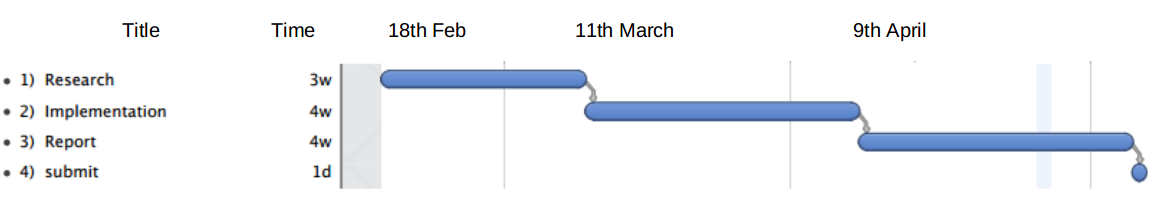
\includegraphics[width=0.9\textwidth]{time-line}
      \caption{Time line for project completion.}
      \label{timline}
  \end{figure}

  For this project to be successful I am planning on spending the initial weeks researching relevant literature and becoming familiar with the concepts of Particle Swarm Optimisation. This is a completely new field to me and understanding the key ideas and models will be critically important. Not only will I need to understand PSO's background I will also need to study previous implementations and applications in order to become absolutely comfortable with it. Finally, as I am planning on improving an existing algorithm, I will have to spend some time becoming familiar enough with the code so that I will be able to modify it with ease.

  The implementation stage will consist of designing the future system and the realisation of the plans. Key design decisions will have to be made during this stage and the solutions might be obtained from the analysis of previous work. 

  To complete this project test driven development will be carried out. I plan to test after every implementation or modification. This will be done to ensure that changes will not affect any previous functionality. The tests will evaluate the efficiency as well as the accuracy of my system. Given the nature of PSO's `random' initialisation,  I want to make sure that the results are consistent. 

  The writing of this result will be flexible, the sections will be written as needed or when the section arises naturally throughout the project. 

  % section methodology (end)

  \section{Technology} % (fold)
  \label{sec:technology}

    \subsection{Haskell} % (fold)
    \label{sub:haskell}
      Coming from a strong mathematical background I find functional languages easier to understand. Also one huge advantage of pure functional languages is that the absence of side-effects allow them to offer a clear semantic framework to analyse the correctness of programs. 

      As Haskell is the functional language I am more familiar with, I did not see the point in learning a new language as it would only restrict my project process, so Haskell was a clear winner. 

      There are other PSO implementations in other languages such as C and Ruby but as already mentioned, Haskell is my preferred language. 

    % subsection haskell (end)
    \subsection{Operating System} % (fold)
    \label{sub:operating_system}
    As Haskell is platform independent (in the sense that it can be compiled in Windows, Linux or Mac) I have chosen to use Ubuntu 12.04 as it is my preferred OS and I feel the most comfortable with it. In addition, I would not be affected in the about of software needed for the project as it is provided for all three OSs already mentioned. 

    The work was carried out on my personal laptop (Intel CORE$^{TM}$ i3 @ 2.6GHZ,4Gb RAM). If required due to any reasons, the university provide classroom PCs (Intel CORE$^{TM}$ i3-2100 CPU @3.10 GHz, 3 Gb RAM) although I have faith that my own machine will be reliable enough for me not to have to change machines. 
    
    Sublime Text 2 was chosen as the IDE for the project. It has many useful functions \cite{sublime} and similarly for the choice of OS, I am happy with this editor.
    % subsection operating_system (end)
  
  % section technology (end)

\chapter{System Design and Architecture}

  \section{Original PSO Implementation} % (fold)
  \label{sec:original_pso_implementation}
    \subsection{Initialisation} % (fold)
    \label{sub:initialisation}
    The main purpose of this stage is to create a population of particles (called a swarm) which will be used to search the domain and find the optimal solution to our problem. The application uses a function called \textit{initialise} to randomly create a list of initial particles to populate the search space. It is written in accordance with Algorithm~\ref{eq:pso} and thanks to Haskell's well designed and efficient random generators \cite{random} it ensures that the particles are initialised in such a way to exploit the search space well. For details, see Algorithm~\ref{eq:pso}. After the population has been initialised, the algorithm moves on to the optimisation phase.
    % subsection initialisation (end)
    \subsection{Inertia Weights} % (fold)
    \label{sub:inertia_weights}
    PSO relies on randomness, as in Equation~\ref{eq:vel}. As this project is not intended to experiment much with the basic PSO parameters we will use the inertia weights presented in \cite{constriction_factor_3}. If there is enough time, we may wish to experiment with different weights. This does not mean that testing will not be done, it just means that we will not deviate from our goal to look into this matter, as so much research has already been done\cite{inertia}.
    % subsection inertia_weights (end)
    \subsection{Optimisation} % (fold)
    \label{sub:optimisation}
    This is done by ``steps'', at each ``step'' a particle is updated by a function \textit{updateParticle} in accordance to Equation~\ref{eq:vel} which changes the position and velocity. The same function checks whether the new position is better that the best solution so far. A boolean system is used, if the new position of the particles is better that global best position, if it is then it changed the global best to this new global best. This is done recursively until all the particles in the swarm have been updated. Function had to be created to deal with the comparison of particles' results and both the position and the value of that position are stored for each particle. 

    For any more details on how the optimisation is done, please refer to \nameref{sec:particle_swarm_optimisation} in Chapter 2.
    % subsection optimisation (end)
    \subsection{Termination} % (fold)
    \label{sub:termination}
    An function was created to deal with the termination, a user specifies the number of iterations (``steps'') that the algorithm is allowed to run for. This independent function is simple, it runs recursively, applying one \textit{updateParticle} at a time and terminates once there are no more iterations to be performed and returns both the value of the global best and it's position. 
    % subsection termination (end)
  % section original_pso_implementation (end)

  \section{Expansion for Portfolio Optimisation} % (fold)
  \label{sec:expansion_for_portfolio_optimisation}

    \subsection{Interface and User Input} % (fold)
    \label{sub:interface_and_user_input}
    The original implementation needed the swarm size and number of iterations to be hard-coded into the algorithm. This model allows the user to specify how many particles they would like as well as how many iterations the PSO should run for. I do not think the user should be allowed to set the inertia weights and they might not fully understand their purpose and therefore give un-optimised inputs. 
    % subsection interface_and_user_input (end)
    % ----------------------------------------------------
    % \subsection{Optimisation} % (fold)
    % \label{sub:optimisation}
    
    % % subsection optimisation (end)
    % ----------------------------------------------------
    \subsection{Constriction Factor} % (fold)
    \label{sub:constriction_factor}
    Maurice Clerc in his study on stability and convergence of PSO \cite{constriction_factor} has introduced the concept of a constriction factor. Clerc indicated that the use of a constriction factor may be necessary to insure convergence of the PSO for certain fitness functions.

    In order to ensure convergence of the PSO, the velocity from Equation~\ref{eq:vel} can be expressed as follows:

    \begin{equation} \label{eq:cf}
      \begin{split}
        V_{i}^{t+1} & = K \Bigg[ V_{i}^{t} + c_1 r_1 \times \Big( Pbest_{i}^{t} - X_{i}^{t} \Big) + c_2 r_2 \times \Big( Gbest^{t} - X_{i}^{t} \Big) \Bigg] \\
        \text{where }\\
        K & = \frac{2}{\mid 2 - \phi - \sqrt{\phi^2 -4\phi} \mid} \text{ and } \phi = c_1 + c_2 \text{ s.t. } \phi > 4  \\
        % \text{and} \\
        % \phi = c_1 + c_2 , \phi > 4 \\
      \end{split}
    \end{equation}

    The convergence characteristic of the system can be controlled by $\phi$ through choosing suitable $c_1$ and $c_2$ in \eqref{eq:cf}. In this approach, $\phi$ must be greater than 4 to guarantee stability \cite{constriction_factor_2}.
    % subsection constriction_factor (end)
    \subsection{Termination} % (fold)
    \label{sub:termination}
    If time allows, it would be nice to have a self-termination PSO which, no matter how many iterations are left, terminates if it thinks that the optimal solution is reached. This could be done by the concept of a threshold, if all the solution reach this threshold, then there is no point in carring of. For example, if all the solution are close enough to each other for a long period of iteration, say $10^{-10}$, then there is no point in looking for thousands more iterations just to find something which will not affect the outcome. 
    % subsection termination (end)
    \subsection{Fitness Function} % (fold)
    \label{sub:fitness_function}
    Due to the nature of Haskell and with some mathematical background it is almost trivial to create a function to represent the measure of risk, namely $\rho_{a,p}(R)$ in Equation~\ref{eq:portfolio-risk} in Section~\nameref{sec:portfolio_management} Chapter~\ref{chap:background}. What is much more challenging is finding a way to include the constraints in Equation~\ref{eq:portfolio-risk-constraints} in a way that the algorithm can deal with the main function without violating these condition. Two methods were considered, using multi-objective optimisation or a penalty function. Due to the constraints being linear-independent, it will be straight forward to affect the optimal solution through factors of the constraints. The design of this will be described in the following Subsection~\ref{sub:penalty_function}.
    % subsection fitness_function (end)
    \subsection{Penalty function} % (fold)
    \label{sub:penalty_function}
    
    % subsection penalty_function (end)
    \subsection{Presenting the Results} % (fold)
    \label{sub:presenting_the_results}
    After the algorithm has finished, the results are displayed on the screen and saved in a separate file which will be called ``output-DATE'', where date is in (year,month,day) format, for example ``output-2014,3,15''. If there is multiple runs in one day, the new results are added to the end of that same file.
    % subsection presenting_the_results (end)
  % section expansion_for_portfolio_optimisation (end)


\chapter{Financial Data}
  \section{Data Description} % (fold)
  \label{sec:data_description}
  
  % section data_description (end)

  \section{Problem Domain} % (fold)
  \label{sec:problem_domain}
  
  % section problem_domain (end)

  \section{Assets and their Weights} % (fold)
  \label{sec:assets_and_their_weights}
  
  % section assets_and_their_weights (end)

  \section{Analysis} % (fold)
  \label{sec:analysis}
  
  % section analysis (end)

  \section{PSO Parameters} % (fold)
  \label{sec:pso_parameters}
  
  % section pso_parameters (end)

  \section{Experimentation and Testing} % (fold)
  \label{sec:experimentation_and_testing}
  
  % section experimentation_and_testing (end)

  \section{Portfolio Constraints} % (fold)
  \label{sec:portfolio_constraints}
  
  % section portfolio_constraints (end)

  \section{Results} % (fold)
  \label{sec:results}
  
  % section results (end)


\chapter{Experimentation and Testing}

  \section{Efficiency} % (fold)
  \label{sec:efficiency}
    Standard Deviation stuff, box plots blahh blahhh
  % section efficiency (end)

  \section{Constriction Factors} % (fold)
  \label{sec:constriction_factors}
  In System Design and Architecture~\ref{sub:constriction_factor} the concept of a constriction factor was introduced. 
    
    \subsection{Testing Strategy} % (fold)
    \label{sub:testing_strategy}
      I plan to test whether this will in fact affect the outcome of the algorithm when applied to the portfolio optimisation problem, furthermore if it does affect it, then whether it improves or worsens the result. In order to test this I will conduct six different experiments, three without a constriction factor where one has the adjustment parameters taken from \cite{constriction_factor_3}, one with the two randomness coefficients that add up to less than 4 and one where they add up to more than 4, the importance of 4 can be read in \cite{constriction_factor}. Then three more with a constriction factor and the rest is the same as the previous three.

      All tests will run 20 times and the results and the time taken will be recorded, all tests will be set to 50 particles, 500 iterations and 10 assets. A mean result and standard deviation will be computed to be able to compare the results. This will give enough indication on how the constriction factor affects the fitness function and how it differs under various criteria.  
    % subsection testing_strategy (end)

    \subsection{Hypothesis} % (fold)
    \label{sub:hypothesis}
      Constriction factor when applied to the portfolio selection problem with appropriate coefficients will not improve the portfolio selection problem.
    % subsection hypothesis (end)

    \subsection{Results} % (fold)
    \label{sub:results}
      This subsection shows the results and the following Table~\ref{table:constriction_factor_results} contains the exact values for the results in my experiment, it will follow a short explanations of the results. 

      Firstly, the time it took for each test to run and there was no significant difference between them. Having a constriction factor did not affect the time it takes for the algorithm to complete. 

        \begin{table}[H]
          \setlength{\extrarowheight}{2.0pt}
          \begin{tabular}{|l|l|l|}
            \hline
            Test & Mean Result & Standard deviation \\
            \hline
            WO-CF Pefersen & 0.914099 & $1.61088\times10^{-16}$ \\
            \hline
            WO-CF $<$ 4 & 0.914099 & $1.72748\times10^{-16}$ \\
            \hline
            WO-CF $>$ 4 & 0.9141 & $5.36229\times10^{-6}$ \\
            \hline
            W-CF Pefersen & 0.91415 & 0.0000389374 \\
            \hline
            W-CF $<$ 4 & 0.91416 & 0.0000448388 \\
            \hline
            W-CF $>$ 4 & 0.914099 & $2.81328\times10^{-16}$ \\
            \hline
          \end{tabular}
          \caption{Results for \nameref{sec:constriction_factors}.}
          \label{table:constriction_factor_results}
        \end{table}

      Table~\ref{table:key_constriction_factor_results} shows what the acronyms in Table~\ref{table:constriction_factor_results} mean. 

        \begin{table}[H]
          \setlength{\extrarowheight}{2.0pt}
          \begin{tabular}{ l l }
            WO-CF Pefersen & : Without constriction factor and Pefersen coefficients  \\
            WO-CF $<$ 4 & : Without constriction factor and $\phi < 4$ \\
            WO-CF $>$ 4 & : Without constriction factor and $\phi > 4$ \\
            W-CF Pefersen & : With constriction factor and Pefersen coefficients  \\
            W-CF $<$ 4 & : With constriction factor and $\phi < 4$ \\
            W-CF $>$ 4 & : With constriction factor and $\phi > 4$ \\
          \end{tabular}
          \caption{Key for \nameref{table:constriction_factor_results}.}
          \label{table:key_constriction_factor_results}
        \end{table}

      The reason for using Pefersen coefficients is stated in the design and architecture section of this report, \nameref{eq:cf} in \nameref{sec:original_pso_implementation}. One can see from Table~\ref{table:constriction_factor_results} that importance having $\phi > 4$ when introducing the constriction factor, in W-CF Pefersen and W-CF $<$ 4 one can see a serious decrease in the optimum found. 

      What is interesting here is that PSO for the fitness function is efficient and consistent without the constriction factor as shown in Table~\ref{table:constriction_factor_results} where WO-CF Pefersen and WO-CF $<$ 4 both have the same mean and almost exact standard deviation, meaning they behave the same. Once we introduce the constriction factor, it is almost catastrophic if we do not have $\phi > 4$, as both W-CF Pefersen and W-CF $<$ 4 have less efficient means and huge standard deviations (in comparison to the other tests) meaning they are unstable and unreliable. Once we make $\phi > 4$, the algorithm settles back to normal but does display higher standard deviation. 
    % subsection results (end)
    \subsection{Conclusion} % (fold)
    \label{sub:conclusion}
      Constriction factor when applied to the portfolio optimisation problem does not improve the results as in the hypothesis. It makes the results more unstable, the algorithm will therefore not include a constriction factor. 

      The use of the constriction coefficient can be viewed as a recommendation to the particle to ``take smaller steps''\cite{constriction_factor_4}, because of this it exploits optimal solutions, which is fine if there are not many, but it does mean that it travels less in the same amount of time. This is one of the main reasons why it did not improve the results. One has to bare in mind that each asset adds a dimension to out search space, this increases domain exponentially so as you increase the amount of assets in a portfolio coupled with making the PSO take smaller steps results in a much larger search space and less area covered by the end of the algorithm. 
       
    % subsection conclusion (end)

      % \begin{align}
      %   V_{i}^{k+1} & = K \Bigg[ V_{i}^{k} + c_1 r_1 \times \Big( Pbest_{i}^{k} - X_{i}^{k} \Big) + c_2 r_2 \times \Big(Gbest_{i}^{k} - X_{i}^{k} \Big) \Bigg] \\
      %   \text{where } \\
      %   K & = \frac{2}{\mid 2 - \phi - \sqrt{\phi^2 -4\phi} \mid}  \\
      % \end{align}

  % section constriction_factors (end)

  \section{Scalability} % (fold)
  \label{sec:scalability}

    \subsection{Testing Strategy} % (fold)
    \label{sub:testing_strategy}
      The application will be run

    % subsection testing_strategy (end)

    \subsection{Hypothesis} % (fold)
    \label{sub:hypothesis}
      
    % subsection hypothesis (end)

    \subsection{Results} % (fold)
    \label{sub:results}
      
    % subsection results (end)

    \subsection{Conclusion} % (fold)
    \label{sub:conclusion}
      
    % subsection conclusion (end)

    Number of assets
  % section scalability (end)

  \section{Relationships} % (fold)
  \label{sec:relationships}
  This test might seem a little peculiar at first but be  assure, there is method in this madness, that's what I tell myself anyways... I want to see what the relationship is (if any) between the time it takes to run, number of particles, number of iterations and number of assets.

    \subsection{Testing Strategy} % (fold)
    \label{sub:testing_strategy}
      I will run nine tests and record the time it takes to finish and the results just to make sure they are consistent. Each of the nine tests will be run 20 times with a mean and standard deviation calculated and shown in the following sections. The nine tests will be as follows:
        \begin{itemize}
          \item Test 1: PSO 20 particles, 100 iterations, 5 assets
          \item Test 2: PSO 20 particles, 300 iterations, 5 assets
          \item Test 3: PSO 40 particles, 100 iterations, 5 assets
          \item Test 4: PSO 20 particles, 100 iterations, 7 assets
          \item Test 5: PSO 20 particles, 300 iterations, 7 assets
          \item Test 6: PSO 40 particles, 100 iterations, 7 assets
          \item Test 7: PSO 20 particles, 100 iterations, 10 assets
          \item Test 8: PSO 20 particles, 300 iterations, 10 assets
          \item Test 9: PSO 40 particles, 100 iterat
          ions, 10 assets
        \end{itemize}
    % subsection testing_strategy (end)

    \subsection{Hypothesis} % (fold)
    \label{sub:hypothesis}
    There is no hypothesis here, I hope that there is no exponential relationship between increase in assets to increase in time for PSO to finish. The point of this exercise is to see if anything interesting happens. 
    % subsection hypothesis (end)

    \subsection{Results} % (fold)
    \label{sub:results}
    Sum of weights for all results
    Results mean 1.
    Results standard deviation $1.3735*10^-9, 0., 1.60689*10^-11, 6.4372*10^-9, 2.66467*10^-15, 1.29662*10^-11, 0.027735, 2.28702*10^-11, 2.54305*10^-10$

    Time taken for PSO to finish for all tests
    Results mean 0.0463947, 0.107632, 0.0812466, 0.0555938, 0.1253, 0.106167, 0.089034, 0.181696, 0.17403
    Results standard deviation 0.00487954, 0.00912289, 0.00542592, 0.00491575, 0.00699414, 0.00669427, 0.00856579, 0.00828043, 0.00557404

    Expected Return
    Means:
    0.0447, 0.0447, 0.0447, 0.0527, 0.0527, 0.0527, 0.101475, 0.1007, 0.1007
    Standard Deviation:
    $6.13954*10^-11, 1.58041*10^-17, 7.18283*10^-13, 3.3924*10^-10, 1.41115*10^-16, 6.83323*10^-13, 0.00279292, 2.30303*10^-12, 2.56085*10^-11 $

      
    % subsection results (end)

    \subsection{Conclusion} % (fold)
    \label{sub:conclusion}
      
    % subsection conclusion (end)
  % section relationships (end)

  \section{Scalability Time } % (fold)
  \label{sec:scalability_time }
  This test might seem a little peculiar at first but be  assure, there is method in this madness (or madness in this method!). I want to see what the relationship is between time, number of particles, number of iterations and number of assets.

    \subsection{Testing Strategy} % (fold)
    \label{sub:testing_strategy}
      The application will be run

    % subsection testing_strategy (end)

    \subsection{Hypothesis} % (fold)
    \label{sub:hypothesis}
      
    % subsection hypothesis (end)

    \subsection{Results} % (fold)
    \label{sub:results}
      
    % subsection results (end)

    \subsection{Conclusion} % (fold)
    \label{sub:conclusion}
      
    % subsection conclusion (end)

    Number of assets
  % section scalability Time and  (end)

  \section{Penalty value} % (fold)
  \label{sec:penalty_value}

    \subsection{Testing Strategy}
      The application will be run

    \subsection{Hypothesis}

    \subsection{Results}

    \subsection{Conclusion}
    
    For fitness function
  % section penalty_value (end)

  \section{Asset percentage/Induced/Forced Diversification} % (fold)
  \label{sec:asset_percentage}

    \subsection{Testing Strategy}
      The application will be run

    \subsection{Hypothesis}

    \subsection{Results}

    \subsection{Conclusion}

    Constraint that says you have to invest between 0.05 to 0.35 on each asset
  % section asset_percentage (end)

  \section{Risk and Risk Aversion} % (fold)
  \label{sec:risk_and_risk_aversion}

    \subsection{Testing Strategy}
      The application will be run

    \subsection{Hypothesis}

    \subsection{Results}

    \subsection{Conclusion}

    Level of riskiness
  % section risk_and_risk_aversion (end)



\chapter{Future Work}

  \section{PSO Parameters} % (fold)
  \label{sec:parameters}
    More testing on WPG inertia weights
    Dunno...
  % section parameters (end)

  \section{Self-termination} % (fold)
  \label{sec:self_termination}
    Stops after some criteria is met
  % section self_termination (end)

  \section{Diversification} % (fold)
  \label{sec:diversification}
    One of the most interesting concepts in portfolio theory I found was that of diversification, unfortunately I found this very late into my project and unable, due to time constraints, to include this into my application. Diversification excites me as it contradicts intuition. One would think that if one have one risky asset, adding another one would only increase the overall risk further, in fact it does the exact opposite!

    The most simplistic model to represent this concept is the proverb, ``putting ones eggs in more than one basket''. Regardless on what the probability of each egg is, having more baskets with eggs is more likely to preserve more eggs that less baskets with the same amount of eggs. In other words, if one basket crashes, one still have the the other eggs which where in different baskets. 

    Now something more useful and even less intuitive is that if ones invests in more than one company within the same sector, for example split all ones money equally (for simplicity in example) and invest in all the mobile phone networks there are. Now company $x$ gets into trouble for some reason which affects the stock market (fraud, IT, quality etc.) and the stock price for $x$ begins to fall, ones will find that the price of stocks for all the other companies goes up. This is due to the investors and business which was with company $x$ now deciding to opt out of that company and therefore bringing more investors and business to all the other companies in the market. 

    My application has a sense of diversification due to the extra constraint which I added late in the project as a emergency diversification solution. It states that one must invest between 5\% and 35\% on each asset to force diversification. This is vaux or brute intelligence though, what could be useful if the application gives a little extra preference if it knows that some assets belong to the same sector. 

  % section diversification (end)
  
  \section{Asset's Covariance} % (fold)
  \label{sec:covariance}
    Risk in terms of 
  % section covariance (end)

  \section{Market Relationships} % (fold)
  \label{sec:market_relationships}
    Gold vs Money
  % section market_relationships (end)

    This would be brilliant!!

  \section{Real-time processing} % (fold)
  \label{sec:real_time_processing}
    Wow!
  % section real_time_processing (end)


\chapter{Discussion and Conclusion}

  \section{Discussion} % (fold)
  \label{sec:discussion}
  
  % section discussion (end)

  \section{Future Work} % (fold)
  \label{sec:future_work}
  
  % section future_work (end)

  \section{Conclusion} % (fold)
  \label{sec:conclusion}
  
  % section conclusion (end)

\bibliographystyle{plain}
\bibliography{myref}

\chapter*{Appendix A: User Manual}

\chapter*{Appendix B: Maintenance Manual}

\end{document}